\section{Material Design}
Because we want our app to look decent, our path will be guided by material design.
What is material design?
Material design is a systematic approach and set of guidelines for creating UI.
It describes individual components, when to use them and when to not use them.
The description includes proportions, behaviour and color system.

\section{The three main screens}
From specifications, it's clear that we need at least one screen for execution history, one for pipelines and one for settings.
On the android platform, there are multiple navigation designs.

\subsection{Navigation drawer}
The hamburger icon at the top left and sliding menu from left to the right.
If you have 5 or more top level screens, or if you want to have some sort of hierarchical menu, this might be the right choice for you, but that's not our case. We have only three main screens.
Also, with the increasing sizes of mobile phones and most people being right-handed, it's hard to reach the hamburger menu with your right thumb.

\subsection{Tabs}
Slidable tabs on top of the screen.
Recommendation for this type of navigation is at least two screens.
You can click on tab names or you can just slide left or right in order to navigate between the screens.
For now, it is one possibility.

\subsection{Bottom navigation}
Three to five icons, usually with text, at the bottom of the screen.
It solves the annoying problem with short thumb, because you no longer need to reach the top left corner with it.
Material design states, that the recommended number of links is three to five. That sounds good.
It is another possibility.

%\subsection{Bottom navigation}
%Three to five icons, optionally with text, at the bottom of the screen.
%It solves the annoying problem with short thumb, because you no longer need to %reach the top left corner with it.
%Material design states, that the recommended number of links is three to five. %That sounds good.
%For now, it is one possibility.
%
%\subsection{Tabs}
%Slidable tabs on top of the screen.
%Recommendation is at least two screens.
%You can click on tab names or you can just slide left or right in order to %navigate between the screens.
%It is another possibility.
%
%\subsection{Conclusion}
%The choice is either bottom navigation or tabs.
%I'm choosing tabs, because I like the idea of having an option to slide between the screens, rather than to be forced to only click.

\subsection{Conclusion}
The choice is either bottom navigation or tabs.
And the winner is bottom navigation because we will be displaying some lists of items on those screens. We will make those items swipeable, but we can't have swipeable items on top of swipeable navigation, that would be a mess.

%\begin{figure}
%	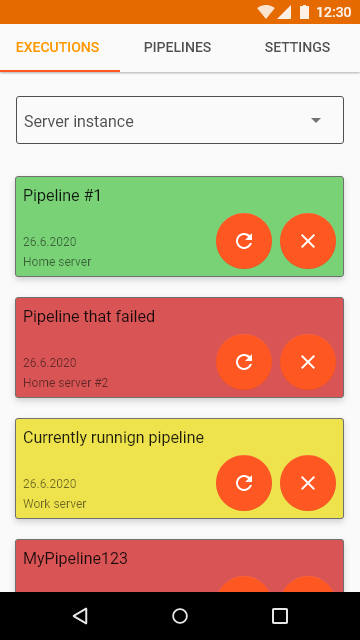
\includegraphics[width=0.3\textwidth]{pics/xd/History.png}
%	\caption[History]{History screen design}\label{fig:xdHistory}
%	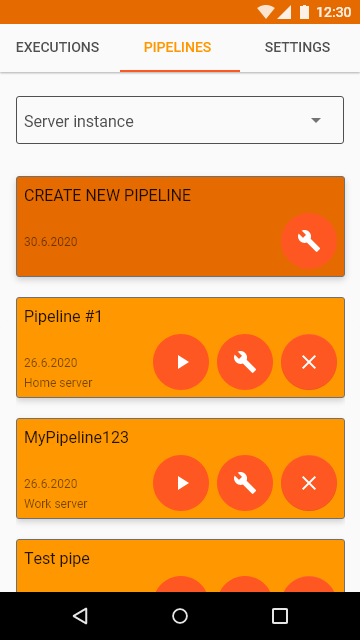
\includegraphics[width=0.3\textwidth]{pics/xd/Pipelines.png}
%	\caption[Pipelines]{Pipelines screen design}\label{fig:xdPipelines}
%	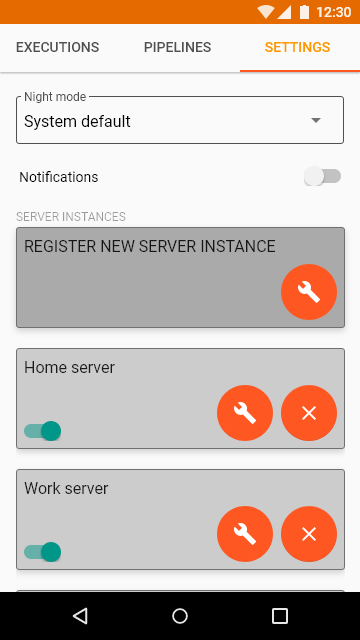
\includegraphics[width=0.3\textwidth]{pics/xd/Settings.png}
%	\caption[Settings]{Settings screen design}\label{fig:xdSettings}
%\end{figure}

\begin{figure}\centering
    \begin{minipage}[b]{0.32\textwidth}
    	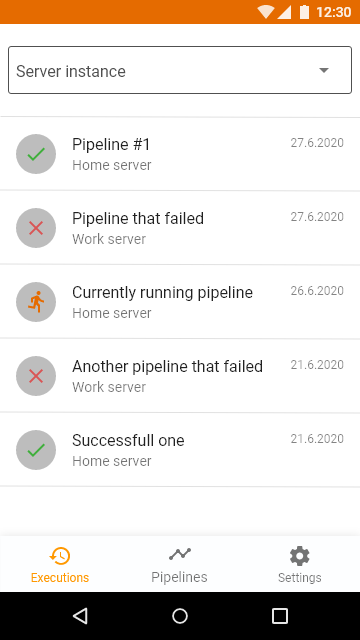
\includegraphics[width=\textwidth]{pics/xd/Bottom Navigation - executions.png}
    	\caption[History]{History screen design}\label{fig:xdHistory}
    \end{minipage}
    \begin{minipage}[b]{0.32\textwidth}
    	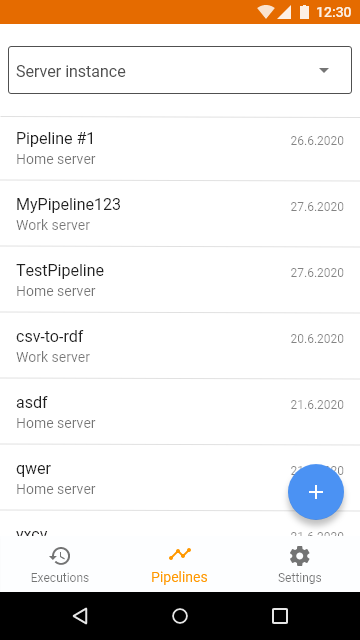
\includegraphics[width=\textwidth]{pics/xd/Bottom Navigation - pipelines.png}
    	\caption[Pipelines]{Pipelines screen design}\label{fig:xdPipelines}
    \end{minipage}
    \begin{minipage}[b]{0.32\textwidth}
    	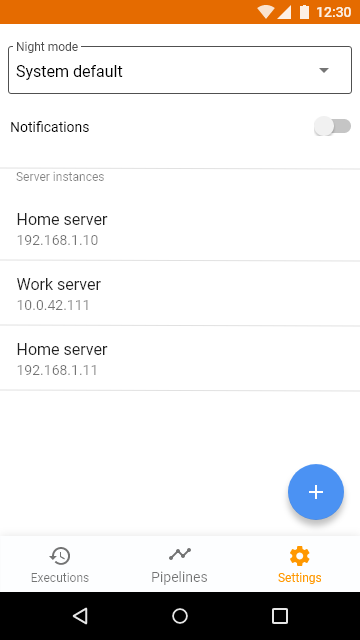
\includegraphics[width=\textwidth]{pics/xd/Bottom Navigation - settings.png}
    	\caption[Settings]{Settings screen design}\label{fig:xdSettings}
    \end{minipage}
\end{figure}

\subsection{Lists}
Each of the three main screens will display some sort of list.
For execution screen it's list of executions, for pipeline screen it's list of pipelines and for settings screen it's list of server instances.

All of those lists will have one thing in common and that being the swipe gesture.
When you swipe an item to left or right, it will be deleted.
User will have the ability to undo this operation for a short period of time.

Tapping on item from execution screen or from pipeline screen will launch the pipeline.
Long click on item from the pipeline screen will open the edit pipeline screen.

\begin{figure}\centering
    \begin{minipage}[b]{0.32\textwidth}
    	\includegraphics[width=\textwidth]{pics/xd/Bottom Navigation - pipelines – 1.png}
    	\caption[Deleting pipeline]{Deleting pipeline design}\label{fig:xdDeletePipeline}
    \end{minipage}
    \begin{minipage}[b]{0.32\textwidth}
    	\includegraphics[width=\textwidth]{pics/xd/Bottom Navigation - pipelines – 2.png}
    	\caption[Undo option]{Undo option design}\label{fig:xdUndo}
    \end{minipage}
\end{figure}

\section{Another screens}
The three main screens are obviously not the only screens our app will consists of.

\subsection{Edit server instance}
While registering new server instance or editing an already registered one, the app needs the address for communication and some name for better organising.
We will also let the user add some description on the instance, so he doesn't need to store everything he wants to store about the instance in the server name.
There could also be some option to ping the server (F-2.6) to verify the address and a way to cancel the registration/edit.
Because of this all, we want to add another screen just for registering/editing server instance.

\begin{figure}\centering
    \begin{minipage}[b]{0.32\textwidth}
    	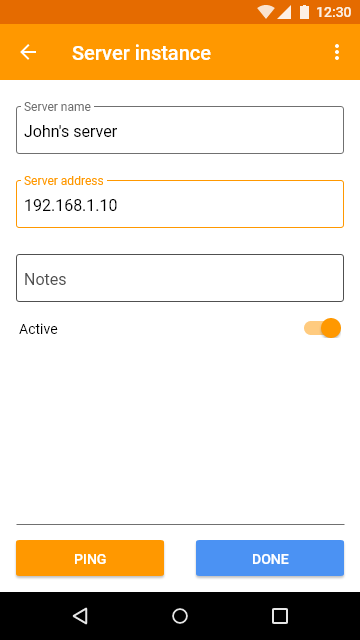
\includegraphics[width=\textwidth]{pics/xd/Edit server instance.png}
    	\caption[Edit server instance]{Edit server instance screen design}\label{fig:xdEditServerInstance}
    \end{minipage}
\end{figure}

\subsection{Edit pipeline screen}
As F-4.2 states, there have to be a screen for editing pipelines.
Short description: This is the screen displaying pipeline components and drawing links between them.

\begin{figure}\centering
    \begin{minipage}[b]{0.32\textwidth}
    	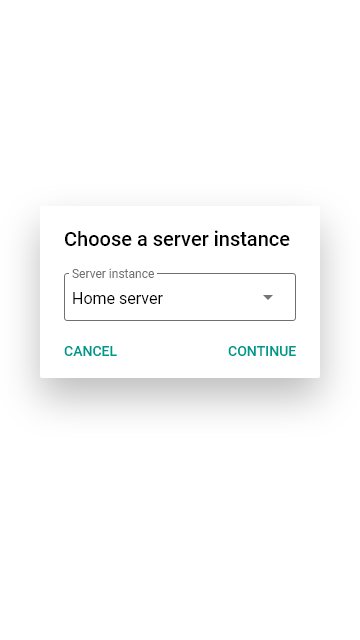
\includegraphics[width=\textwidth]{pics/xd/Create new pipeline.png}
    	\caption[Create new pipeline dialog]{Create new pipeline dialog design}\label{fig:xdCreateNewPipelineDialog}
    \end{minipage}
    \begin{minipage}[b]{0.32\textwidth}
    	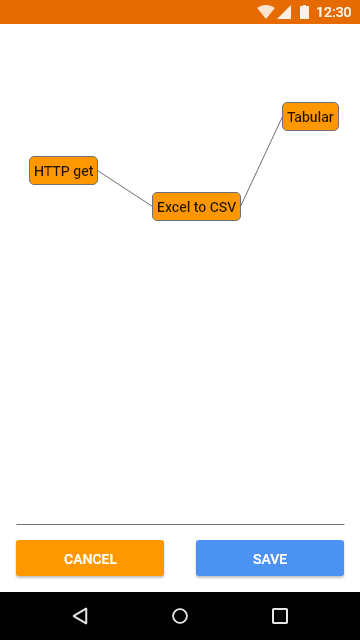
\includegraphics[width=\textwidth]{pics/xd/Pipeline editor.png}
    	\caption[Edit pipeline screen]{Edit pipeline screen design}\label{fig:xdPipelineEditor}
    \end{minipage}
\end{figure}



\subsection{Edit component screen}
Each component have it's own settings so there is a need for another screen.

\begin{figure}\centering
    \begin{minipage}[b]{0.32\textwidth}
    	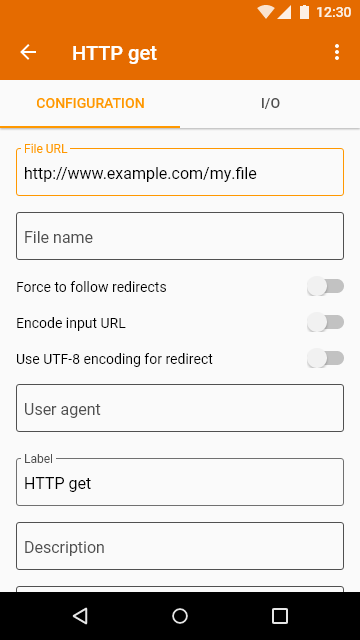
\includegraphics[width=\textwidth]{pics/xd/Edit component - configuration.png}
    	\caption[Edit component screen 1]{Edit component screen 1 design}\label{fig:xdEditComponent1}
    \end{minipage}
    \begin{minipage}[b]{0.32\textwidth}
    	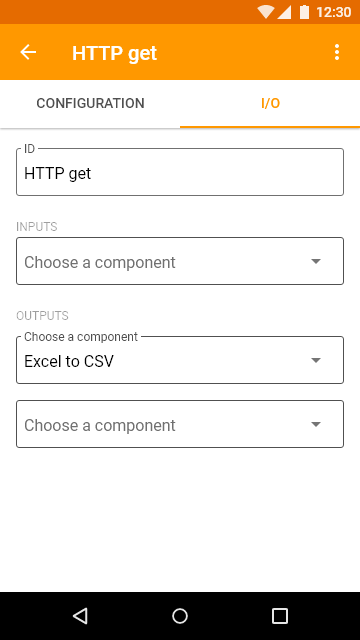
\includegraphics[width=\textwidth]{pics/xd/Edit component - io.png}
    	\caption[Edit component screen 2]{Edit component screen 2 design}\label{fig:xdEditComponent2}
    \end{minipage}
\end{figure}

%\begin{figure}\centering
%    \begin{minipage}[b]{0.32\textwidth}
%    	\includegraphics[width=\textwidth]{pics/xd/Edit unsupported component - %configuration.png}
%    	\caption[Edit unsupported component screen 1]{Edit unsupported %component screen 1 design}\label{fig:xdEditUnsupportedComponent1}
%    \end{minipage}
%    \begin{minipage}[b]{0.32\textwidth}
%    	\includegraphics[width=\textwidth]{pics/xd/Edit unsupported component - %io.png}
%    	\caption[Edit unsupported component screen 2]{Edit unsupported %component screen 2 design}\label{fig:xdEditUnsupportedComponent2}
%    \end{minipage}
%\end{figure}

\subsection{Notifications}
Requirements engineering tells us, we need to implement notifications.

\begin{figure}\centering
    \begin{minipage}[b]{0.7\textwidth}
    	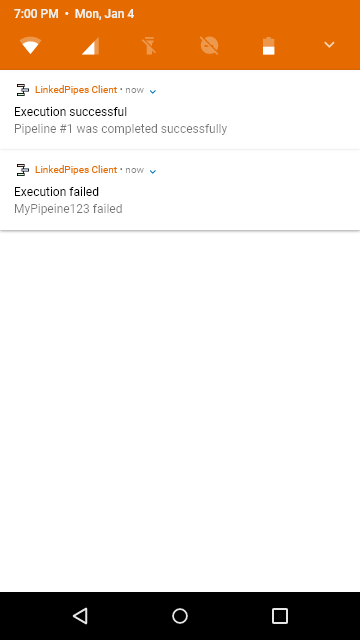
\includegraphics[width=\textwidth]{pics/xd/Notifications.png}
    	\caption[Notifications]{Notification design}\label{fig:xdNotifications}
    \end{minipage}
\end{figure}